\documentclass{article}

% Packages
\usepackage{geometry}
\usepackage{graphicx}
\usepackage{lipsum}
\usepackage{listings}
\usepackage[portuguese]{babel}

% Page setup
\geometry{a4paper, margin=2cm}

\begin{document}

% cover
\thispagestyle{empty} % Remove page number from first page

\begin{figure}[t]
    
\includegraphics[width=3cm]{images/logo-puc-minas.png}
    \hspace{0.02\textwidth}
    \vline%
    \hspace{0.04\textwidth}
    
\includegraphics[width=3cm]{images/logo-icei.jpeg}
\end{figure}

\hrulefill%
\vspace{\baselineskip}

\Large\noindent
\textbf{Pontifícia Universidade Católica de Minas Gerais} \\
\textbf{Instituto de Ciências Exatas e Informática} \\
\textbf{Departamento de Engenharia de Computação}

\begin{center}
    \vfill
    \Huge\textbf{Relatório: Trabalho Prático 2} \\
    \vspace{0.5cm}
    \Large\textbf{Registradores em VHDL} \\
    \vspace{1cm}
    \large \textbf{Professor(es)}: Antônio Hamilton Magalhães\\
    \vspace{0.5cm}
    \large \textbf{Aluno(s)}: Bruno Luiz Dias Alves de Castro \\
    \large \hspace{0.75cm} Rafael Ramos de Andrade \\
    \vfill
    \large Belo Horizonte \\ Campus Coração Eucarístico \\
    \vspace{\baselineskip}
    \large \today
\end{center}

% table of contents
\newpage
\thispagestyle{empty}
\tableofcontents

% body
\newpage
\large % document text size

\section{Introdução}

Durante as aulas da disciplina de Sistemas Reconfiguráveis, fomos introduzidos à linguagem VHDL. VHDL (\textbf{V}HSIC \textbf{H}ardware \textbf{D}escription \textbf{L}anguage) é uma linguagem de descrição de hardware. Com ela, podemos montar circuitos lógicos de maneira totalmente textual, o que garante à linguagem uma grande vantagem ante à soluções visuais.

\subsection{Objetivos}

\subsection{Simulação via Quartus II}

Nessa etapa realizamos testes no software Quartus II da altera.

\subsubsection{Bloco w\_reg}

Nesta imagem é realizado 3 testes para verificar a funcionalidade do registrador, nos primeiros 60ns é alterado os bits da entrada de dados (d\_in) para nivel lógico alto, o bit de reset (nrst) que é ativo em baixa, é desativado, ou seja, nível lógico alto e o bit de ativação (wr\_en) é colocoado em nível lógico alto após 10ns. Assim é possível verificar a mudança na saída (w\_out) com um tempo de delay de 6ns. No segundo teste a partir de 60ns até 140ns é resetado os bits da memória do registrador colocando reset em nível lógico zero, o resultado é propagada para a saída após o tempo de delay de aproximadamente 6ns. No terceiro teste foi verificados se o bit de ativação de escrita está funcionando corretamente, portanto com o bit 6 da saída em nível lógico alto esse valor será escrito apenas no tempo 160ns quando é colocado a porta de ativação do registrador em nível lógico alto e o registrador é escrito.

\begin{figure}[ht]
\begin{center}
    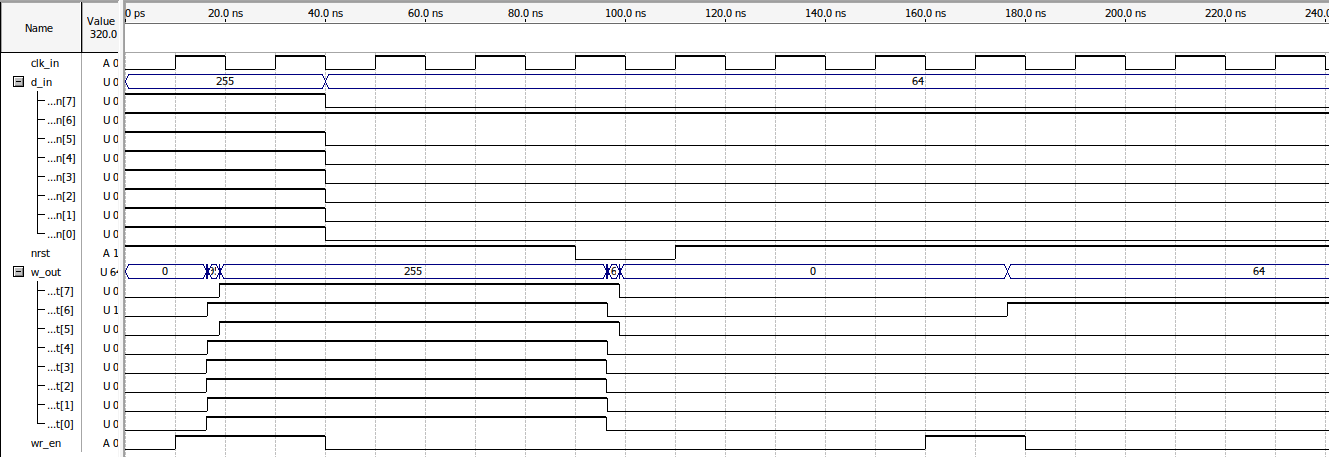
\includegraphics[width=15cm]{images/w_reg.png}
    \caption{Simulação bloco w\_reg}
\end{center}
\end{figure}

\section{Conclusão}
Com estes dois projetos simples, tivemos um excelente primeiro contado com a linguagem VHDL, bem como à programação concorrente e desenvolvimento de circuitos FPGA. Os dois circuitos implementados (Multiplexador de Endereçamento e Unidade Lógica Aritimética) são blocos de construção chave para a maior parte dos circuitos complexos, e serão de suma importância não só para os demais trabalhos práticos que realizaremos ao longo do semestre, mas para nosso desenvolvimento acadêmico e profissional.

\end{document}
